\section{Why to use parallel programming?}
\begin{frame}[fragile]
  \frametitle{Why to use parallel programming?}
  \begin{itemize}
  \item Until 2005, CPU frequency kept doubling every year or so and your old sequential program would automatically run faster on the new hardware without you having to do anything.
  \item This is no longer true: we cannot keep increasing CPU frequency since we cannot handle so much heat per unit area.
  \item As a result, during recent decade the progress in computing hardware was in increasing degree of parallelism by using wider vectors, 
    more CPU cores, offloading computations to accelerators such as GPUs, TPUs, FPGAs, using faster memory, 
    increasing bandwidth between memory and CPU or CPU and accelerators, 
    using faster interconnect between nodes in a cluster to be utilized, for example, by MPI or other distributed computing framework.
  \item Your old sequential program will not run any faster on the new hardware unless 
    you redesign it to utilize the available parallelism.
  \item Offloading part of computation to GPU is one way to speed up your program, potentially by $10^n$.
  \end{itemize}
\end{frame}

\begin{frame}
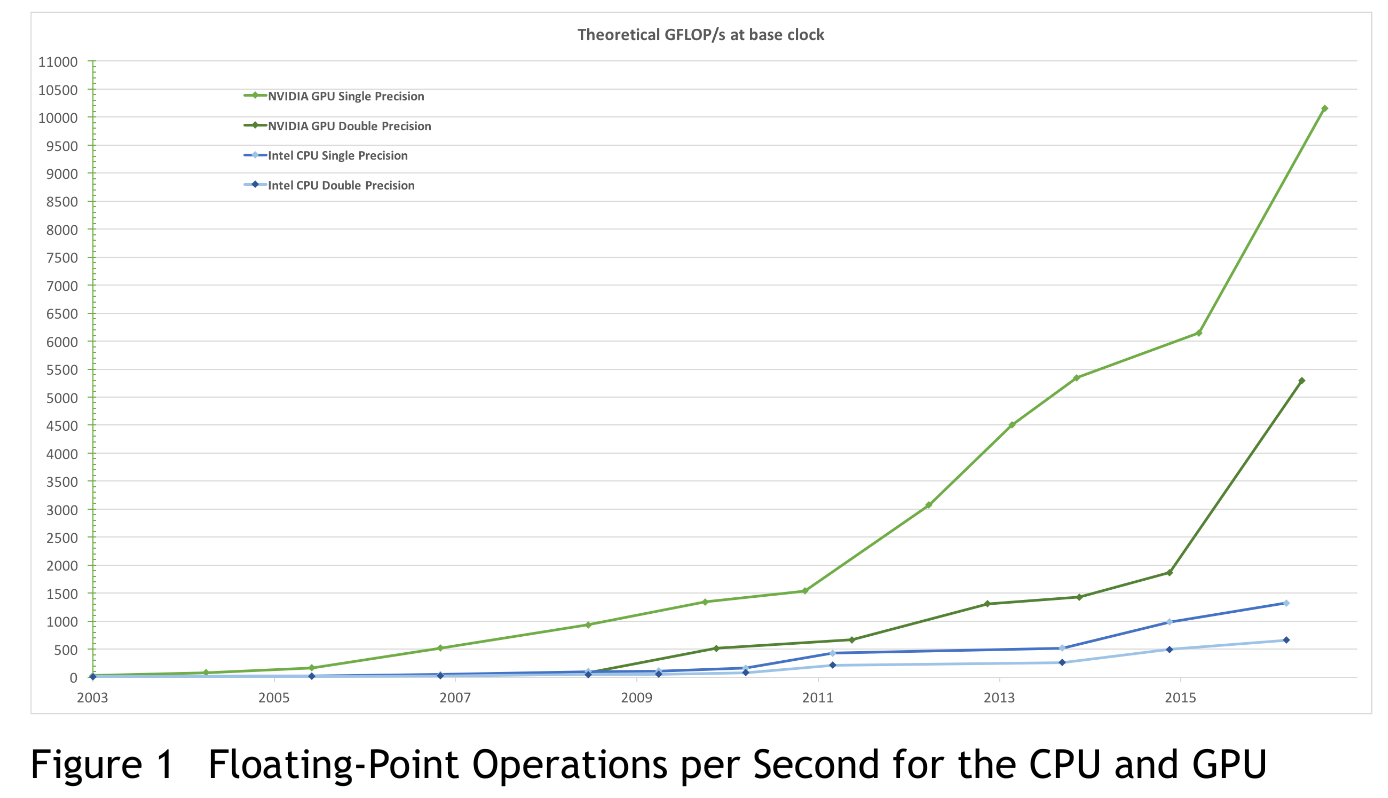
\includegraphics[width=11.5cm]{graphs/fps.png}
\end{frame}


\begin{frame}
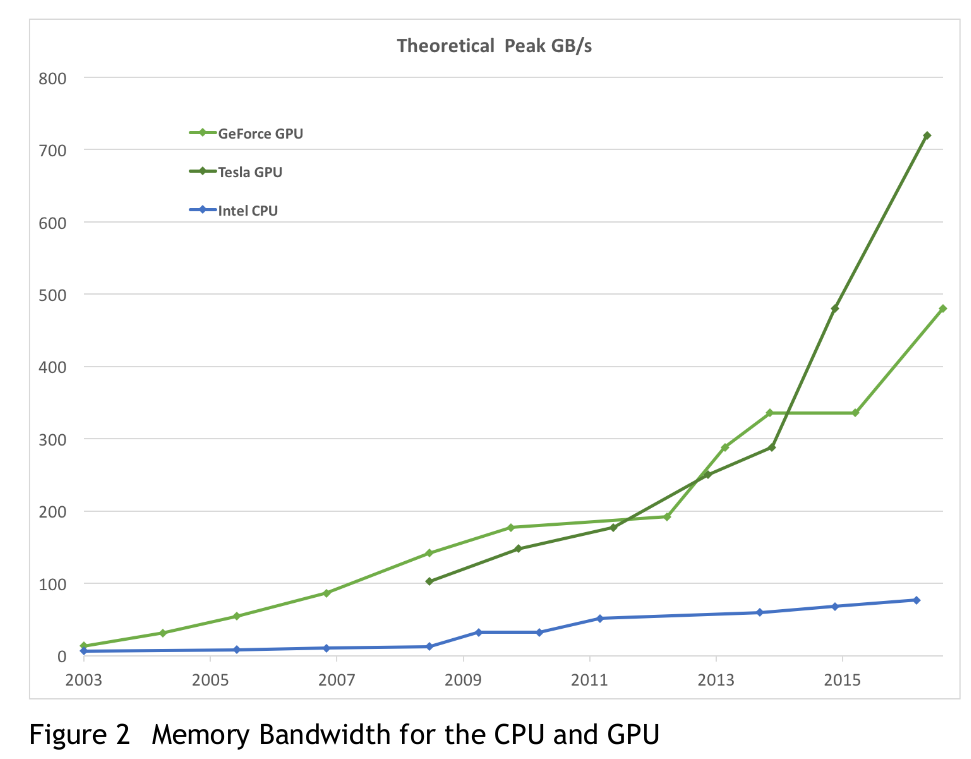
\includegraphics[width=11.5cm]{graphs/bps.png}
\end{frame}
